\chapter{免疫防御}\label{ch:g9:immune-defenses}

门户已守住（\cref{prop:g9:microbes-and-infection:doors}）
——然而有时仍有入侵者登陆：木刺
带来的\omterm{def:g9:microbes-and-infection:sorted}{细菌}在温暖的组织中增殖，\omterm{def:g9:microbes-and-infection:sorted}{病毒}已在
气道\omterm{def:g5:first-look-at-cells:cell}{细胞}内大量复制。接下来登场的是
身体继\omterm{def:g8:nervous-communication:neuron}{神经}与\omterm{def:g8:hormonal-communication:glands}{激素}之后的第三大系统：
\omterm{def:g9:immune-defenses:memory}{免疫}防御——一支常备军、一支带有记忆的专业部队，
以及提前对其进行训练的
\omterm{prop:g9:immune-defenses:vaccination}{接种疫苗}这一手段。

\section{快速反应：炎症}

\begin{definition}[常备军]\label{def:g9:immune-defenses:standing}
在\omterm{prop:g4:journey-of-food:absorb}{血液}和组织中巡逻的是白
\omterm{def:g5:first-look-at-cells:cell}{细胞}\index{白细胞}——\omterm{def:g9:immune-defenses:memory}{免疫}系统的士兵，
在骨髓中产生，循着
\cref{prop:g4:heart-and-blood:carries}的网络流动。
最先赶到的是\emph{吞噬\omterm{def:g5:first-look-at-cells:cell}{细胞}}：
能流动着包围入侵者并将其\omterm{def:g4:journey-of-food:digestion}{消化}
（\cref{ex:g6:cell-unit-of-life:drop}中流动的变形虫
与独立生活的捕食者用的是同一招式——机体
把这一古老的本领用作防御）。
\end{definition}

\begin{proposition}[正确理解炎症]\label{prop:g9:immune-defenses:inflammation}
木刺扎伤后的表现——发红、发热、肿胀、
搏动痛，并非\omterm{def:g9:microbes-and-infection:stages}{感染}占了上风，而是防御
正在赶来。受损组织发出的警报信号使
局部\omterm{def:g4:heart-and-blood:vessels}{血管}扩张（\cref{prop:g7:organs-at-work:supply}
中的改道与征用）：更多温热\omterm{prop:g4:journey-of-food:absorb}{血液}涌入，\omterm{def:g4:heart-and-blood:vessels}{血管}壁
渗漏，吞噬\omterm{def:g5:first-look-at-cells:cell}{细胞}从\omterm{def:g7:heart-and-circulation:vessels}{毛细血管}中挤出，
爬向病灶，一路吞食\omterm{def:g9:microbes-and-infection:sorted}{细菌}。脓液
是战场的“战报”——耗尽的吞噬\omterm{def:g5:first-look-at-cells:cell}{细胞}、
死去的入侵者与碎屑。多数入侵在数日内
悄然平息，无人察觉。
\end{proposition}
\admitted

\begin{example}[解读愈合中的伤口]\label{ex:g9:immune-defenses:cut}
第一天：红、热、压痛的红晕——\omterm{def:g4:heart-and-blood:vessels}{血管}扩张，
援军到达。第二天：少量脓液——战报。第四天：
红晕消退，结痂干燥——增殖败给了
吞噬作用，\omterm{def:g1:the-five-senses:sense}{皮肤}的重建
（\cref{prop:g5:first-look-at-cells:growth}）随即关上
身后的大门。整场战役在
未及引起担忧之时便已打赢。
\end{example}

\section{专门部队：识别与记忆}

\begin{proposition}[特异性免疫应答]\label{prop:g9:immune-defenses:specific}
当快速反应跟不上时，专门部队
登场——速度较慢，但更加精准：
\begin{itemize}
  \item 每种入侵者都带有表面标记——它的
        \emph{抗原}\index{抗原}——一种分子
        形状，专门\omterm{def:g5:first-look-at-cells:cell}{细胞}借此识别外来物（
        “自身”标记与
        \cref{ex:g9:unique-individuals:medicine}中的识别方式相同，
        只是方向转向体内）；
  \item 在专门的\omterm{def:g9:immune-defenses:standing}{白细胞}中，少数带有
        与\emph{此种}\omterm{prop:g9:immune-defenses:specific}{抗原}相契合的受体；接触
        即将其筛选出来，它们增殖为克隆大军
        （选择的逻辑在体内数日内运行）；
  \item 它们的武器：\emph{抗体}\index{抗体}
——注入\omterm{prop:g4:journey-of-food:absorb}{血液}的专用分子，能
        结合并聚集入侵者，供吞噬\omterm{def:g5:first-look-at-cells:cell}{细胞}清除——
        以及杀伤性\omterm{def:g5:first-look-at-cells:cell}{细胞}，摧毁机体自身已被劫持的
        \omterm{def:g5:first-look-at-cells:cell}{细胞}，这是阻止\omterm{def:g9:microbes-and-infection:sorted}{病毒}“复制机器”的唯一办法，
        （见\cref{ex:g9:microbes-and-infection:contrast}）；
  \item 战斗的代价也是疾病的一部分：
        发热（身体有意升温——许多
        \omterm{prop:g9:microbes-and-infection:mostly}{病原体}在温热时繁殖更差）、酸痛、
        肿大的\emph{淋巴结}——专门部队的
        营房，战时拥挤不堪。
\end{itemize}
\end{proposition}
\admitted

\begin{definition}[免疫记忆]\label{def:g9:immune-defenses:memory}
胜利之后，部分克隆大军转入
\emph{记忆细胞}\index{记忆细胞}：长寿的
专门\omterm{def:g5:first-look-at-cells:cell}{细胞}，保存着\omterm{prop:g9:immune-defenses:specific}{抗原}的特征信息。若
\emph{同一}入侵者再次登陆，遇到的是有准备的部队
——数小时内作出应答，症状出现之前便清除入侵者：
你便获得\emph{免疫}\index{免疫}。麻疹一生只得一次，
不会两次；去年冬天的毒株无法再点燃
今年的疫情。
（见\cref{pb:g9:microbes-and-infection:1}）。记忆
解释了为何同一种感冒似乎不会来两次，也
解释了为何感冒仍不断出现：其\omterm{def:g9:microbes-and-infection:sorted}{病毒}\omterm{prop:g9:genes-and-dna:explains}{突变}很快
（\cref{prop:g9:genes-and-dna:explains}）变成
记忆所不持有的特征描述。
\end{definition}

\section{训练防御：接种疫苗}

\begin{proposition}[接种疫苗]\label{prop:g9:immune-defenses:vaccination}
\emph{接种疫苗}\index{接种疫苗}即
在无病的情况下建立的\omterm{def:g9:immune-defenses:memory}{免疫}记忆：向专门\omterm{def:g5:first-look-at-cells:cell}{细胞}
展示入侵者的\emph{特征描述}——灭活或减毒的
\omterm{def:g9:microbes-and-infection:sorted}{微生物}、携带\omterm{prop:g9:immune-defenses:specific}{抗原}的无害片段——
整个选择与记忆的程序便会运行，只是
没有危险。受训的部队日后若遇到真正的
\omterm{prop:g9:microbes-and-infection:mostly}{病原体}，即为第二次登陆。
公共\omterm{def:g1:healthy-habits:hygiene}{卫生}方面有两点重要后果：
\begin{enumerate}
  \item 接种者在首次交战之前便已受到保护，
        这对于首次交战即可致死或致残的疾病
        至关重要；
  \item 足够多的已接种邻居可使疫情“断粮”
——缺乏可\omterm{def:g9:microbes-and-infection:stages}{感染}的宿主，
        （\cref{pb:g9:microbes-and-infection:1}中
        的消退）：保护是共享的——这层屏障
        也覆盖那些太小或病弱、无法自行
        接受训练的人。
\end{enumerate}
\end{proposition}
\admitted

\begin{example}[从牛痘豪赌到根除天花]\label{ex:g9:immune-defenses:history}
这段历史始于詹纳 1796 年的豪赌——挤奶女工
\omterm{def:g9:microbes-and-infection:stages}{感染}轻微牛痘却从未染上天花；一次牛痘接种
便训练出对抗这一杀手的\omterm{def:g9:immune-defenses:memory}{免疫}力——历经
巴斯德刻意减弱\omterm{def:g9:microbes-and-infection:sorted}{微生物}制成的疫苗
（\cref{ex:g9:microbes-and-infection:history}中的作者，
完成了他的理论），直至二十世纪的
点名：天花，人类古老的祸患，
\emph{被根除}——该\omterm{def:g9:microbes-and-infection:sorted}{病毒}自 1970 年代末起
在野外已\omterm{prop:g5:biodiversity:loss}{灭绝}，而\omterm{def:g5:brain-in-command:system}{脊髓}灰质炎被逼入
地图上最后的角落。汇集起来的训练记忆，
是迄今唯一消灭过人类疾病的武器。
\end{example}

\begin{omfigure}
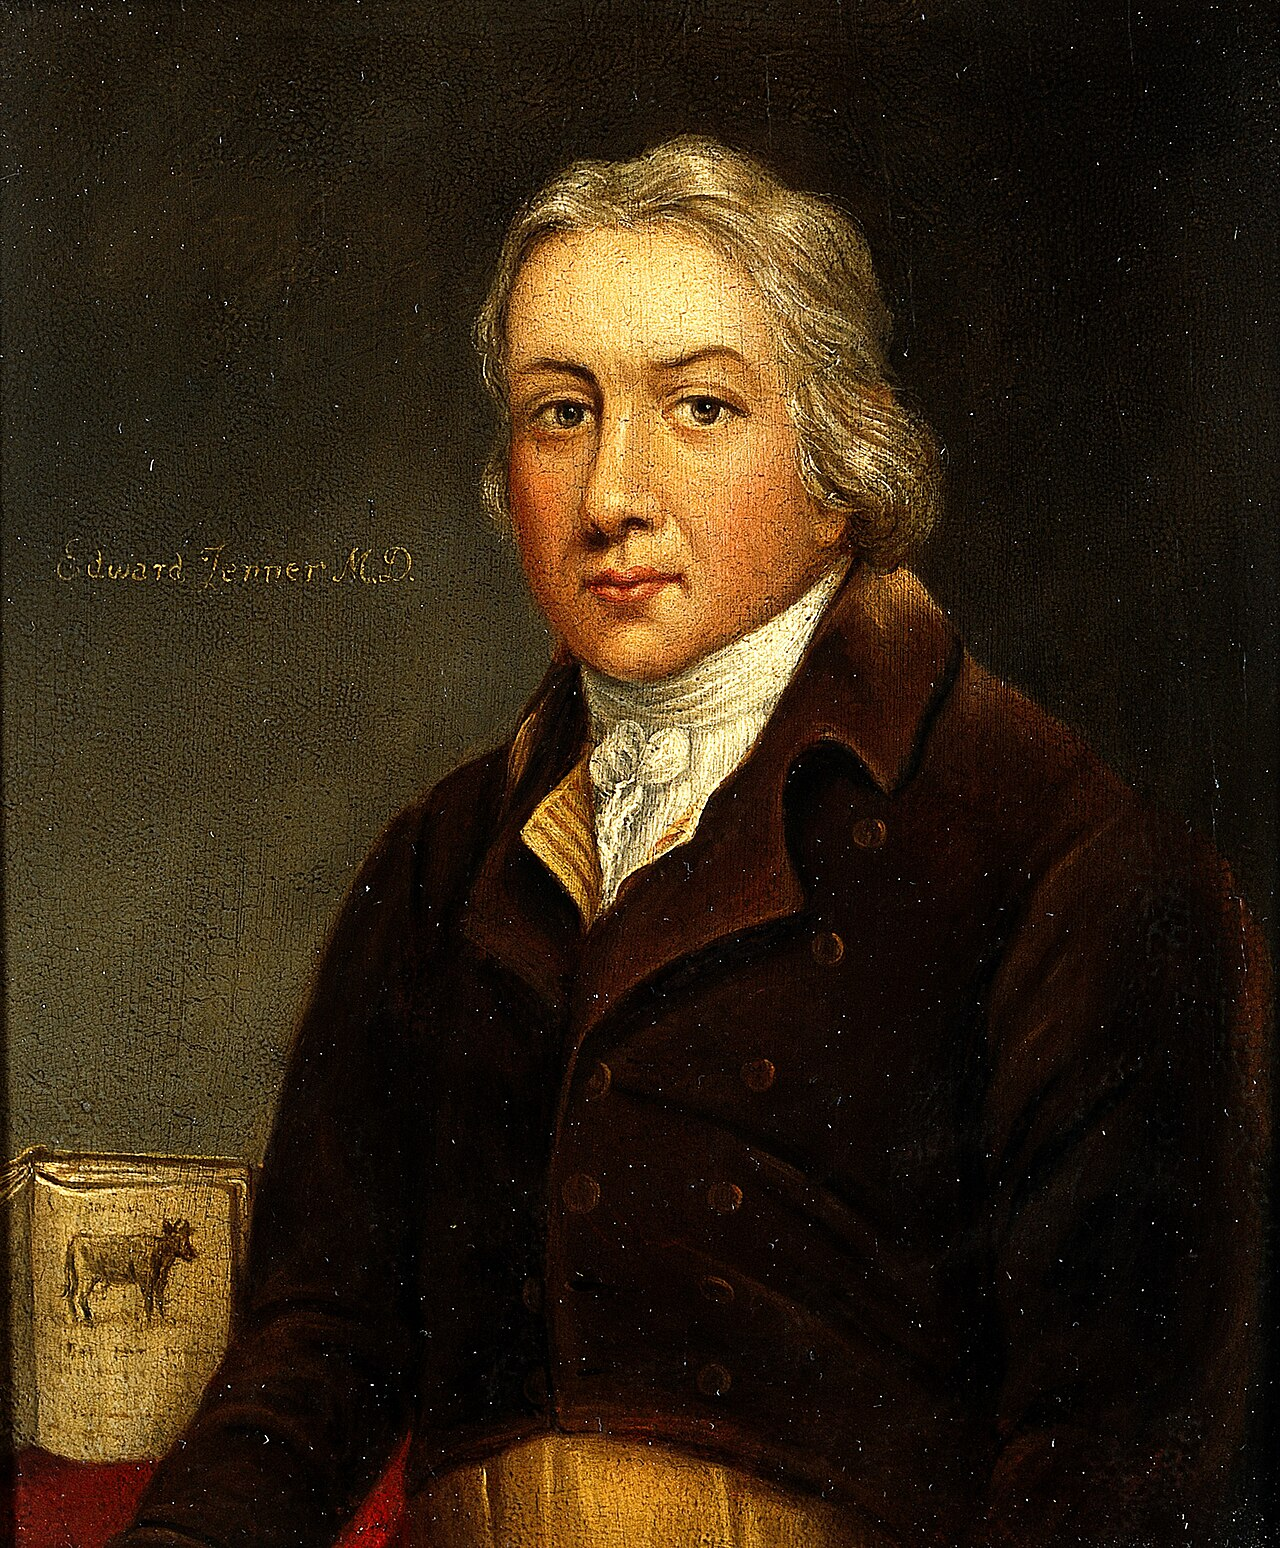
\includegraphics[width=0.46\linewidth]{images/book1/jenner.jpg}

{\small 爱德华·詹纳，主持了 1796 年的牛痘豪赌，
由此发展出疫苗接种。油画，Wellcome Collection，
CC~BY~4.0.}
\end{omfigure}

\begin{method}[解读任何免疫事件]\label{met:g9:immune-defenses:read}
对于任何\omterm{def:g9:microbes-and-infection:stages}{感染}、康复、疫苗或检测结果：
\begin{enumerate}
  \item 判断此次相遇：是首次侵入还是再次侵入？
        （记忆改变一切）；
  \item 指出应答者：吞噬\omterm{def:g5:first-look-at-cells:cell}{细胞}的快速应答、
        特异性\omterm{def:g9:immune-defenses:memory}{免疫}\omterm{def:g5:first-look-at-cells:cell}{细胞}的克隆大军，或常备记忆；
  \item 正确解读征象：炎症与发热
        是防御在起作用，肿大的淋巴结即是兵营；
  \item 对于疫苗：识别所呈递的
        \omterm{prop:g9:immune-defenses:specific}{抗原}描述，以及它汇集的是谁的保护。
\end{enumerate}
\end{method}

\section{练习}

\begin{exercise}[$\star$]\label{exo:g9:immune-defenses:1}
常备军和最先应答的\omterm{def:g5:first-look-at-cells:cell}{细胞}是谁，
它们分别产生于何处？
\end{exercise}

\begin{exercise}[$\star$]\label{exo:g9:immune-defenses:2}
把木刺伤口的四种征象译为防御事件。
\end{exercise}

\begin{exercise}[$\star$]\label{exo:g9:immune-defenses:3}
什么是\omterm{prop:g9:immune-defenses:specific}{抗原}、\omterm{prop:g9:immune-defenses:specific}{抗体}，以及二者之间的
联系？
\end{exercise}

\begin{exercise}[$\star$]\label{exo:g9:immune-defenses:4}
为什么在\omterm{def:g9:microbes-and-infection:sorted}{病毒}\omterm{def:g9:microbes-and-infection:stages}{感染}中，杀伤性特异性\omterm{def:g9:immune-defenses:memory}{免疫}\omterm{def:g5:first-look-at-cells:cell}{细胞}必须
摧毁机体自身的\omterm{def:g5:first-look-at-cells:cell}{细胞}？
\end{exercise}

\begin{exercise}[$\star$]\label{exo:g9:immune-defenses:5}
什么是\omterm{def:g9:immune-defenses:memory}{记忆细胞}？第二次侵入时，
会遇到什么？
\end{exercise}

\begin{exercise}[$\star$]\label{exo:g9:immune-defenses:6}
用一句话给\omterm{prop:g9:immune-defenses:vaccination}{接种疫苗}下定义，句中须用
“描述”与“记忆”。
\end{exercise}

\begin{exercise}[$\star\star$]\label{exo:g9:immune-defenses:7}
为什么发热是一种武器而非故障——
它利用了哪条先前的\omterm{def:g6:exploring-our-environment:conditions}{条件}规则？
\end{exercise}

\begin{exercise}[$\star\star$]\label{exo:g9:immune-defenses:8}
“麻疹一次，绝不两次——感冒却屡屡复发。”
请用
\cref{def:g9:immune-defenses:memory}解释两句话。
\end{exercise}

\begin{exercise}[$\star\star$]\label{exo:g9:immune-defenses:9}
特异性\omterm{def:g5:first-look-at-cells:cell}{细胞}的克隆大军，即“在体内进行的
选择”。请将这一类比对应到
\cref{prop:g9:how-species-change:selection}中的三条
事实。
\end{exercise}

\begin{exercise}[$\star\star$]\label{exo:g9:immune-defenses:10}
请解释汇集起来的保护——以及依赖它的是谁——
结合疫情的消退加以说明。
\end{exercise}

\begin{exercise}[$\star\star$]\label{exo:g9:immune-defenses:11}
运用\cref{met:g9:immune-defenses:read}分析下列情形：(a) 生锈钉子扎伤后的
破伤风加强针；(b) 咽喉剧痛时
颈部淋巴结肿大。
\end{exercise}

\begin{exercise}[$\star\star\star$]\label{exo:g9:immune-defenses:12}
以本书的风格撰写天花讣告：\omterm{def:g9:microbes-and-infection:sorted}{病毒}的
致病机制，训练记忆如何将其围堵，
汇集的保护如何终结它——以及为何根除
就是\omterm{prop:g5:biodiversity:loss}{灭绝}（\cref{prop:g5:biodiversity:loss}），
这一原理一次站到了人类一边。
\end{exercise}

\section{问题：疫苗接种台账}

\begin{problem}[{周末问题——卫生保健中心的
一周，用免疫方法解读}]\label{pb:g9:immune-defenses:1}
某\omterm{def:g1:healthy-habits:hygiene}{卫生}保健中心（虚构）的一周：周一，婴儿
\omterm{prop:g9:immune-defenses:vaccination}{接种疫苗}；周二，农夫被生锈铁丝划伤后的
加强针；周三，一名未\omterm{prop:g9:immune-defenses:vaccination}{接种疫苗}的
儿童\omterm{def:g9:microbes-and-infection:stages}{感染}麻疹，并排查其接触者；周四，\omterm{prop:g4:journey-of-food:absorb}{血液}检测
读取\omterm{prop:g9:immune-defenses:specific}{抗体}水平；周五，全体员工的年度
流感疫苗。

\medskip\noindent\textbf{第一部分——本周的病例。}
\begin{enumerate}
  \item 周一的婴儿接受减毒\omterm{def:g9:microbes-and-infection:sorted}{微生物}滴剂
        和片段注射。指出所呈递的是什么，
        并说明接下来几周进行的是哪种
        \omterm{def:g9:immune-defenses:memory}{免疫}程序？
  \item 周二的农夫：伤口要清洗（这属于
        哪一道防线？），并接种加强针。
        \emph{加强针}对已训练过的\omterm{def:g9:immune-defenses:memory}{记忆
        细胞}有何作用——为何在所有疾病中，
        唯独破伤风不允许在首次交战时“赌一把”？
  \item 周三的麻疹患儿：首次入侵，启动完整
        \omterm{def:g9:immune-defenses:memory}{免疫}程序。梳理病程：快速应答
        被超越，克隆大军集结，\omterm{def:g7:organs-at-work:recovery}{恢复}——以及
        随之解除的是什么？
  \item 经排查的接触者分为三类：已\omterm{prop:g9:immune-defenses:vaccination}{接种疫苗}的
        （安然无恙），早已康复者（安然无恙），
        以及一名未\omterm{prop:g9:immune-defenses:vaccination}{接种疫苗}的婴儿，需密切观察。
        对每一类接触者，用
        \cref{met:g9:immune-defenses:read}的第一个问题
        逐一解读。
\end{enumerate}

\medskip\noindent\textbf{第二部分——检测数据。}
\begin{enumerate}[resume]
  \item 周四的检测读取了针对既往疾病
        与疫苗的\omterm{prop:g9:immune-defenses:specific}{抗体}水平。一个较高的\omterm{prop:g9:immune-defenses:specific}{抗体}水平
        能证明什么，它暗示了怎样的
        \omterm{def:g5:first-look-at-cells:cell}{细胞}储备？
  \item 某位患者在\omterm{prop:g9:immune-defenses:vaccination}{接种疫苗}多年后，
        \omterm{prop:g9:immune-defenses:specific}{抗体}水平已经下降，医生开具了加强针。
        请从\omterm{def:g9:immune-defenses:memory}{记忆细胞}的角度解释\omterm{prop:g9:immune-defenses:specific}{抗体}水平
        下降与加强接种的原因。
  \item 周五的流感疫苗需要\emph{每年}接种，
        不同于周一一次或两次接种的方案。流感\omterm{def:g9:microbes-and-infection:sorted}{病毒}
        的哪种特性
        （见\cref{def:g9:immune-defenses:memory}）迫使
        每年都要重新训练\omterm{def:g9:immune-defenses:memory}{免疫}系统？
  \item 为什么\omterm{def:g1:healthy-habits:hygiene}{卫生}保健中心要对\emph{员工}格外强调接种？（谁的
        保护会汇聚于何处，
        在充满病患与体弱者的
        楼宇之中？）
\end{enumerate}

\medskip\noindent\textbf{第三部分——台账的
含义。}
\begin{enumerate}[resume]
  \item 未\omterm{prop:g9:immune-defenses:vaccination}{接种疫苗}的麻疹患儿的父母曾
        畏惧疫苗，信赖“自然”的
        首次交战。请草拟医生温和的
        算账：比较训练\omterm{def:g9:immune-defenses:memory}{免疫}的代价与
        麻疹首次交战的代价。
  \item 那名需重点观察的婴儿年龄太小，
        尚不能\omterm{prop:g9:immune-defenses:vaccination}{接种疫苗}。请说明本应
        保护它的人是谁，这项责任在
        \cref{prop:g9:immune-defenses:vaccination}中称作什么。
  \item 请将周二与周三的情况，对应到两位
        历史人物（见
        \cref{ex:g9:immune-defenses:history}）：
        每次问诊中各体现了谁的思路？
  \item 以一句话为本周台账作结：
        \omterm{def:g1:healthy-habits:hygiene}{卫生}保健中心实际施用的是什么，
        用本章的术语表述。
\end{enumerate}
\end{problem}
